\chapter{Судалгааны хэсэг}
\label{Chapter2} % Энэ бүлэг рүү ишлэл хийх бол \ref{Chapter2} командыг ашигла 
\pagecolor{white}

%-------------------------------------------------------------------------------
%	SECTION 1
%-------------------------------------------------------------------------------
\section{Прокси дахин шифрлэлт}
Прокси дахин шифрлэлт нь нийтийн түлхүүрээр шифрлэсэн өгөгдлийг дахин шифрлэж өөр хувийн түлхүүрээр тайлах боломжийг олгодог.

Мамбо болон Окамото шифрийг тайлан дараа нь шифрлэх уламжлалт аргыг сайжруулах зорилгоор анх гаргаж ирсэн.

1998 онд Blaze, Bleumer, Strauss (BBS) нар "atomic proxy cryptography" гэсэн ойлголтыг санал болгосон бөгөөд үүнд хагас итгэмжлэгдсэн прокси нь үндсэн энгийн текстийг харалгүйгээр Алисын шифрийг Бобын шифр текст болгон хувиргадаг. El Gamel дээр суурилсан схем ба прокси буюу гуравдагч талийн тусламжтайгаар шифрийг дамжуулах зорилготой. \cite{ateniese2005improved}

Прокси дахин шифрлэлт үйл явц нь гурван хэсгээс тогтоно.
\begin{itemize}
    \item \textbf{Төлөөлөгч:} Прокси дахин шифрлэлт ашиглан шифрийг тайлах эрхээ өөр хүнд шилжүүлэх өгөгдлийн эзэн. Дахин шифрлэлтийн түлхүүр үүсгэж, прокси руу илгээдэг. Төлөөлөгчийг ихэвчлэн “Алис” гэж нэрлэдэг.
    \item \textbf{Орлгоч:} Төлөөлөгчийн шифрийг тайлах эрхтэй хүн. Ихэвчлэн "Боб" гэдэг нэртэй байдаг.
    \item \textbf{Прокси:} Дахин шифрлэх шифрийг дамжуулах гуравдагч тал.
\end{itemize}

\textbf{Прокси дахин шифрлэлт үндсэн хоёр төрөлтэй.}
\begin{itemize}
    \item Нэг чиглэлт (Unidirectional PRE)
    \item Хоёр чиглэлт (Bidirectional PRE)
\end{itemize}
Мөн олон дахин шифрлэх боломжтой болон нэг удаагийн шифрлэх боломжтой гэж хуваадаг.

Прокси дахин шифрлэх схем дараах хэсгүүдээс тогтоно.
\begin{itemize}
    \item \textbf{Нийтийн параметрүүд:} Нийтлэг нийтэд байдаг параметрүүд. Түлхүүрийн урт зэрэг.

    \item \textbf{Нийтийн болон нууц түлхүүрийн хослол:} Хэрэглэгч бүр нийтийн/нууц түлхүүрийг үүсгэдэг. Нийтийн түлхүүрийг нийтэд тавьж, харин хувийн түлхүүр нь зөвхөн хэрэглэгч өөртөө үлдээнэ. Боб Алис руу мессеж илгээхдээ Алисын нийтийн түлхүүрийг ашиглан шифрлэж, Алис түүний хувийн түлхүүрийг ашиглан тайлна.

    \item \textbf{Төлөөлөгчийн түлхүүрүүд:} Хэрэглэгч бүр энд rkAlice→Bob гэж тэмдэглэсэн дурын төлөөлөгчид (дахин шифрлэх) түлхүүр үүсгэж болно. rkAlice→Bob тулд Алис прокси дахин шифрлэлтийн алгоритмыг ашиглан хувийн түлхүүрээ Бобын нийтийн түлхүүртэй хослуулан түлхүүр гаргаж авна. Гаргаж авсан түлхүүрээр дахин шифрлэж төлөөлөгчийн хувийн түлхүүрээр тайлах боломжтой болно.

    \item \textbf{Шифрлэгдсэн текст:} Хэрэглэгч ямар нэгэн нийтийн түлхүүрээр мессежийг (энгийн текст) шифрлэх үед шифр текст үүснэ.
\end{itemize}

Нэг чиглэлт \emph{PRE (KE, RG, E, R, D)} хэсгүүдээс тогтоно.
\begin{enumerate}
    \item Алис, Боб болон Чарли хувийн болон нийтийн түлхүүрийг үүсгэнэ. \emph{(KE)}
    \item Алис Боб-д зориулж өгөгдлөө шифрлэж серверт байршуулна.
    \item Боб Алис-ын өгөгдлийг Чарли-тай хуваацлахын тулд \emph{RE(pkB,skB,pkC,skC∗)} шифрлэж серверт байршуулна. Чарлигийн хувийн заавал шаардахгүй үүсгэж болно.
    \item Боб RE-г ашиглаж үүсгэсэн түлхүүрийг серверт явуулж Алисын файлыг дахин шифрлэж Чарли тайлах боломжтой болно.
\end{enumerate}

\begin{figure}[ht]
    \centering
    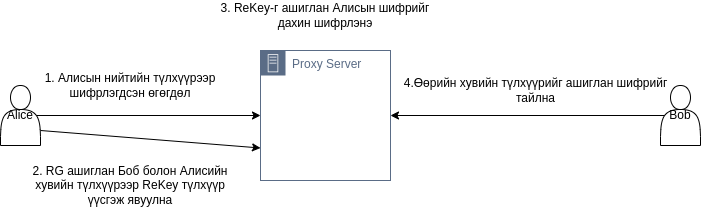
\includegraphics[scale=0.5]{Figures/enencryption_schemes/PRE.drawio.png}
    \caption[Proxy Re-encryption scheme]{Прокси дахин шифрлэх}
    \label{fig:PRE_Scheme}
\end{figure}

Давуу талууд:
\begin{itemize}
    \item Нууцлалыг сайжруулна: PRE нь оролцогч талуудын хувийн мэдээллийг задруулахгүйгээр өгөгдлийг хуваалцахыг зөвшөөрснөөр нууцлалыг сайжруулдаг. Талууд нууцаар эсвэл хувийн нууц мэдээллийг задруулахгүйгээр мэдээллээ хуваалцахыг хүссэн тохиолдолд ашиглах боломжтой.
    \item Илүү уян хатан шифрлэсэн өгөгдлийг өргөн хүрээтэй тараах боломжтой
\end{itemize}

Сул талууд:
\begin{itemize}
    \item Проксид итгэх: PRE нь дахин шифрлэлтийг гүйцэтгэхэд гуравдагч талын прокси дээр тулгуурладаг ба схемийн аюулгүй байдал нь прокси талаас хамаарна.
    \item Хязгаарлагдмал өргөтгөх чадвар: PRE нь өргөтгөх чадварын хувьд хязгаарлагдмал байж болно. Учир нь хэрэглэгчдийн тоо нэмэгдэхийн хэрээр олон талыг дэмжихэд шаардлагатай дахин шифрлэлтийн түлхүүрүүдийн тоо хурдацтай өсөх болно. Энэ нь гол менежментийг төвөгтэй болгож, удирдахад хэцүү болгодог.
    \item Potential for replay attacks: PRE нь халдагч хариуг зогсоож хандах эрхийг өөрт ашигтай солих боломжтой.
    \item Хүчингүй болгоход хүндрэлтэй: PRE дахь өгөгдөлд хандах эрхийг цуцлах нь ялангуяа олон тал оролцсон тохиолдолд төвөгтэй. Хэрэв аль нэг талын дахин шифрлэлтийн түлхүүр алдагдсан бол бусад талуудын мэдээлэлд хандах эрхэд нөлөөлөхгүйгээр өгөгдөлд хандах эрхийг цуцлах нь хэцүү юм.
    \item Хязгаарлагдмал хэрэглээ: PRE нь харьцангуй шинэ бөгөөд шинээр гарч ирж буй технологи хэвээр байгаа бөгөөд илүү уламжлалт шифрлэлтийн схемүүдтэй харьцуулахад хэрэглээ нь хязгаарлагдмал байдаг. Энэ нь технологийг хэрэгжүүлэх, удирдах туршлагатай мэргэжилтнүүд бага байдаг.
\end{itemize}

\subsection*{Прокси дахин шифрлэх схемийн ерөнхий хэрэглээ}
\begin{itemize}
    \item \textbf{Аюулгүй өгөгдөл хуваалцах:} Өгөгдлийн олон хэрлэгчид найдвартай хуваалцахад ашигладаг. Өгөгдлийн эзэмшигч нь өгөгдлийг өөрийн түлхүүрээр шифрлэж, дахин шифрлэж прокси руу шилжүүлдэг. Дараа нь прокси нь хүлээн авагчийн түлхүүрээр шифрлэгдсэн өгөгдлийг хувиргаж, өгөгдөл эзэмшигчийн оролцоогүйгээр шифрийг тайлж, өгөгдөлд хандах боломжийг олгодог.

    \item \textbf{Cloud Storage:} Үүл хадгалах системд хадгалагдсан мэдээллийн аюулгүй байдлыг сайжруулахын тулд прокси дахин шифрлэлтийг ашиглаж болно. Нууц мэдээллийг үүлэн үйлчилгээ үзүүлэгч рүү шууд оруулахын оронд өгөгдлийг эзэмшигчийн түлхүүрээр шифрлэж, прокси түлхүүрээр дахин шифрлэх боломжтой. Дараа нь прокси нь дахин шифрлэгдсэн өгөгдлийг үүлэн дотор хадгалдаг. Энэ нь үүлэн үйлчилгээ үзүүлэгч нь зөвхөн дахин шифрлэгдсэн өгөгдөлд хандах эрхтэй бөгөөд анхны контентыг уншиж чадахгүй байх боломжийг олгодог.

    \item \textbf{Түлхүүр зохицуулалт: (Key escrow)}Түлхүүр эскроу гэдэг нь криптограф түлхүүрийг итгэмжлэгдсэн гуравдагч этгээдэд хадгалах практикийг хэлнэ. Энэ тохиолдолд анхны өгөгдөл нь эзэмшигчийн түлхүүрээр шифрлэгдсэн бөгөөд дахин шифрлэлтийн түлхүүрnийг проксид хадгалагдана. Хэрэв эзэмшигч нь түлхүүрээ алдсан эсвэл өөр төхөөрөмжөөс хандах шаардлагатай бол прокси нь өгөгдлийг шинэ түлхүүрээр дахин шифрлэх боломжтой бөгөөд ингэснээр эзэмшигчид дахин хандах эрх олгоно.

    \item \textbf{Аюулгүй имэйл:} Илгээгч нь хувийн түлхүүрээ шуудангийн сервер эсвэл бусад зуучлагчтай хуваалцахын оронд өөрийн түлхүүрээр имэйлээ шифрлэж, дахин шифрлэх ажиллагааг прокси руу шилжүүлэх боломжтой. Дараа нь прокси нь хүлээн авагчийн түлхүүрээр имэйлийг дахин шифрлэх боломжтой бөгөөд зөвхөн хүлээн авагч нь мессежний кодыг тайлж унших боломжтой.
\end{itemize}

%-------------------------------------------------------------------------------
%	SECTION 2
%-------------------------------------------------------------------------------
\section{Хөгжүүлэх технологи, хэл сонгох}
Прокси дахин шифрлэлт схемийг ашиглан файл хуваалцах систем хөгжүүлэхээр болсон.Хөгжүүлэлтэнд хэрэгтэй хэл болон технологи сонгосон.

Систем хоёр хэсгээс тогтох ба. API сервер болон хэрлэгч талын программ. Пайтон маш олон нэмэлт сангууд байдаг маш том нийгэмлэгтэй (community) хэл. Бичиглэл хялбар олон давуу талтай тул пайтон хэлийг сонгосон.
Үүнд:
\subsubsection*{\textbf{Flask framework}}
Пайтон хэл дээр бичсэн веб хөгжүүлэхэд зориулагдсан  фреймворк юм. Хөнгөхөн олон нэмэлт сан шаардахгүй хэрэгтэй сангуудаа суулгаад хөгжүүлэх боломжтой. Сурахад хялбар өөрийн хүссэн загвараар загварчилж хийх боломжтой. RESTFul API гаргахад хялбар. Хэрэгтэй гэвэл нэмэлт сан ORM зэрэг өөр сангууд суулгаж хамт ашиглах боломжтой.

\begin{lstlisting}[language=Python, caption={Энгийн API үүсгэж буй код}, captionpos=b]
from flask import Flask

app = Flask(__name__)
        
@app.route("/")
    def hello_world():
        return "<p>Hello, World!</p>"
@app.get("/")
    def hello_world():
        return "<p>Hello, get request!</p>"
\end{lstlisting}
app.route endpoint бичих боломжтой маш хялбар мөн хурдан бичих боломжтой.

\subsubsection*{Tkinter}
Хэрэглэгчийн интерфейс (GUI) үүсгэхэд ашигладаг Python номын сан юм. Tcl/TK GUI дээр суурилсан. Линукс виндовс зэрэг олон үйлдлийн системийг дэмждэг. Нэмэлт сангуудтай ажиллах боломжтой.
\begin{lstlisting}[language=Python, caption={Энгийн цонх үүсгэж буй код}, captionpos=b]
import tkinter as tk

root = tk.Tk()
# Create a label widget.
label = tk.Label(root, text="Hello, world!")
# Create a button widget.
button = tk.Button(root, text="Click me!")
# Add the label and button widgets to the root window.
label.pack()
button.pack()
# Start the main loop.
root.mainloop()
\end{lstlisting}
\subsubsection*{pyUmbral}
Прокси дахин шифрлэлтийг файтон дээр хэрэгжүүлсэн пайтоны сан юм. OpenSSL болон Cryptography.io ашиглсан.
\begin{figure}[ht]
    \centering
    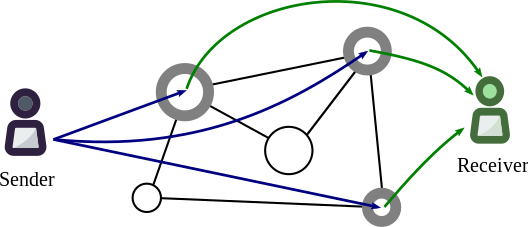
\includegraphics[scale=0.5]{Figures/umbral.png}
    \caption[pyUmbral]{pyUmbral}
    \label{fig:pyUmbral}
\end{figure}

ECIES-KEM болон BBS98 санаа авсан нэг чиглэлтэй дахин шифрлэлтийн сан. pyUmbral функцуудийг ерөнхийд нь гурав ангилсан.
\begin{enumerate}
    \item Түлхүүр үүсгэх алгоритмууд.
          \begin{itemize}
              \item KeyGen()
              \item ReKeyGen(skA, pkB, N, t)
          \end{itemize}
    \item Encapsulation болон Decapsulation
          \begin{itemize}
              \item Encapsulate(pkA)
              \item Decapsulate(skA, capsule)
          \end{itemize}
    \item Re-Encapsulation болон Fragments Decapsulation.
          \begin{itemize}
              \item ReEncapsulation(kF rag, capsule)
              \item DecapsulateFrags(skB, {cF ragi}ti=1, capsule):
          \end{itemize}
\end{enumerate}

\subsubsection*{Фернет (Fernet)}
Тэгш хэмт шифрлэлт  болон баталгаажуулалт хийдэг. 128 битийн түлхүүр бүхий CBC горим дахь AES; PKCS7 ашигладаг. HMAC болон SHA256 баталгаажуулалтанд ашигладаг.

\subsubsection*{Google Cloud Platform}
Гуравдагч тал болох сервер проксиг (API) deploy хийж байршуулах шаардлагатай0. Google Cloud нь маш олон давуу талтай ба үнэгүй туршиж үзэх 300 долларын эрхтэй тул сонгосон.

%-------------------------------------------------------------------------------
%	SECTION 3
%-------------------------------------------------------------------------------
\section{Хөгжүүлэлтийн орчин бэлдэх}
Пайтон хэл нь орчин бүрдүүлэхэд хялбар ба виртуал орчин үүсгэж хэрэгтэй сангуудыг татаж суулгах боломжтой. Бүх линукс тархцад пайтон хэл нь суулгалцан байдаг тул хэрэгтэй сангуудыг татаж суулгахад л хангалтай.

Мөн криптографт ашиглхад сайн хэлнүүдийн нэг ба сангууд нь аюулгүй ашиглахад хялбар.\cite{cryptographyTopLanguaes}

Пайтон хэл дээр хөгжүүлэлт хийхийн тулд прокси дахин шифрлэлтийн сан хэрэгтэй болсон.
JHU-MIT Proxy Re-cryptography Library (PRL) нь хэд хэдэн прокси дахин шифрлэлтийн схемийг хэрэгжүүлсэн нээлттэй эхтэй сан юм. Алгоритмуудыг Жонс Хопкинсийн Их Сургууль болон Массачусетсийн Технологийн Их Сургуулийн судлаачид боловсруулсан бөгөөд Жузеппе Атениезе, Кевин Фу, Мэттью Грин, Сюзан Хохенбергер нарын анхны судалгаанд үндэслэсэн.
JHU-MTI Прокси дахин шифрлэлтийн сан нь C/C++ хэл дээр бичигдсэн байсан. Пайтон хэлний setuptools болон C хэлний "python.h" санг ашиглан пайтоны сан бичих гэж оролдож үзсэн. JHU-MTI сан нь MIRCL санг ашигладаг.

PRL сан нь хоёр схемийг хэрэгжүүлдэг.
\begin{itemize}
    \item \textbf{PRE1:} алгоритм нь Decisional Billinear Diffie-Hellman Assumption (DBDH) дагуу аюулгүй.
    \item \textbf{PRE2:} алгоритм нь Decisional Billinear Inversion Assumption (DBDHI)-ийн дагуу аюулгүй.
\end{itemize}
PRE1 схемийг пайтон сан руу хөрвүүлэх гэж оролдсон.
\subsubsection*{Ерөнхий бүтэц}

\begin{figure}
    \dirtree{%
        .1 ..
        .2 example.
        .3 example.py.
        .2 external.
        .3 miracl.
        .3 proxylib.
        .2 LICENSE.
        .2 README.md.
        .2 setup.py.
        .2 src.
        .3 pypre.cpp.
        .2 userguide.pdf.
    }
    \caption{Модулийн файлын бүтэц}
\end{figure}

\begin{itemize}
    \item \textbf{example} хэсэг тестийн код байрлана.
    \item \textbf{external} хэсэгт PRL сан болон MIRCL сан байна.
    \item Сангуудыг compile хийж \textbf{lib*.a} файл гаргаж авна.
    \item \textbf{setup.py} файл нь тухайн package-ын мэдээлэл байна.
    \item \textbf{pypre.cpp} С++ функцийг нэмэлт сан *.a-аас дуудаж пайтон руу хөрвүүлэх хэсэг.
\end{itemize}

\begin{lstlisting}[language=Python, caption={setup.py}, captionpos=b]
import glob
import os

from setuptools import Extension, setup

os.environ["CC"] = "g++"
os.environ["CXX"] = "g++"

module = Extension(
    "pypre",
    language="c++",
    sources=[f for f in glob.glob('src/*.cpp')]+
    ['external/proxylib/proxylib_pre1.cpp'],
    include_dirs=["external/miracl", "external/proxylib"],
    library_dirs=["external/miracl", "external/proxylib"],
    libraries=["miracl", "proxylib"],
    extra_objects=['external/miracl/libmiracl.a','external/proxylib/libproxylib.a']
)

setup(name='pypre',
      license='Apache',
      author="Myagmartseren",
      author_email='myagmartseren7@gmail.com',
      description='Proxy Re-encryption Python library',
      url='https://github.com/myagmartseren/pre_python',
      ext_modules=[module],
      include_dirs=['external/proxylib','external/miracl'],
)
\end{lstlisting}

\textbf{pypre.py} файл дотор үндсэн C++ кодны санг дуудаж пайтонруу хөрвүүлэх хэсэг байна.
Хэрэгтэй толгой файлыг include хийнэ. Proxylib.h болон miracle гэх мэт сангууд нь setup.py хавсарсан сангууд юм.

\begin{lstlisting}[language=C, caption={pypre.cpp}, captionpos=b]
#define PY_SSIZE_T_CLEAN
#include <zzn.h>
#include <miracl.h>

#include <Python.h>
#include <proxylib.h>
#include <proxylib_pre1.h>    
\end{lstlisting}

\noindent Класс бүрийг C-ын struct-ыг ашиглаж зарлаж өгнө.

\begin{lstlisting}[language=C, caption={pypre.cpp},captionpos=b]
typedef struct
{
    PyObject_HEAD
    ProxyCiphertext_PRE1 *proxyCiphertext_PRE1;
} PyProxyCiphertext_PRE1;
\end{lstlisting}

\noindent Классын method-уудыг зарлаж өгнө. Буцах утга нь хөгжүүлэх функц ашиглана.

\begin{lstlisting}[language=C, caption={generate\_params method}, captionpos=b]
static PyObject* PyPRE1_generate_params(PyObject *self, PyObject *args) {
    if (PyTuple_Size(args) !=1){
        PyErr_SetString(PyExc_RuntimeError, "Should have CurveParams");
        return Py_None;
    }

    PyObject *params = PyTuple_GetItem(args, 0);

    if (!PyCurveParams_Check(params)) {
        PyErr_SetString(PyExc_RuntimeError, "Failed to cast CurveParams");
        return Py_None;
    }

    PyCurveParams *pyParams = (PyCurveParams *)params;

    int result = PRE1_generate_params(*pyParams->params);
    if (!result) {
        PyErr_SetString(PyExc_RuntimeError, "Failed to generate params");
        return PyBool_FromLong(result);
    }

    Py_INCREF(Py_None);
    return PyBool_FromLong(result);
}
\end{lstlisting}

\noindent Бичсэн method-уудыг класст хамааруулна классдаа нэмж өгөн.

\begin{lstlisting}[language=C, caption={generate_params method-г класст хамааруулна.}, captionpos=b]
static PyMethodDef module_methods[] = {
    {"PRE1_generate_params", PyPRE1_generate_params, METH_VARARGS, "Generate curve parameters for the PRE1 scheme."},
    {NULL, NULL, 0, NULL}
};
\end{lstlisting}
\noindent Модулийг зарлаж өгнө. 
\begin{lstlisting}[language=C, caption={Модуль зарлалт}, captionpos=b]
static struct PyModuleDef module_def = {
    PyModuleDef_HEAD_INIT,
    "pypre",
    0,  // m_doc
    -1, // m_size
    module_methods,// m_methods
    /*
    NULL,                 // m_reload
    NULL,                 // m_traverse
    NULL,                 // m_clear
    NULL                  // m_free
    */
};

\end{lstlisting}

\noindent Модулийг import хийх үед классууд зарлаж өгнө.

\begin{lstlisting}[language=C, caption={Модуль нь init хийхэд зарлах классууд}, captionpos=b]
PyMODINIT_FUNC PyInit_pypre(void);

PyObject *PyInit_pypre(void)
{
    extern PyTypeObject PyProxyPK_PRE1Type;
    if (PyType_Ready(&PyProxyPK_PRE1Type) < 0)
        return NULL;

    Py_INCREF(&PyProxyPK_PRE1Type);
    if (PyModule_AddObject(module, "PK_PRE1", (PyObject *)&PyProxyPK_PRE1Type) < 0)
    {
        Py_DECREF(&PyProxyPK_PRE1Type);
        Py_DECREF(module);
        return NULL;
    }

    extern PyTypeObject PyProxySK_PRE1Type;
    if (PyType_Ready(&PyProxySK_PRE1Type) < 0)
        return NULL;

    Py_INCREF(&PyProxySK_PRE1Type);
    if (PyModule_AddObject(module, "SK_PRE1", (PyObject *)&PyProxySK_PRE1Type) < 0)
    {
        Py_DECREF(&PyProxySK_PRE1Type);
        Py_DECREF(module);
        return NULL;
    }
    // PyModule_AddObject(module, "__version__", PyUnicode_FromString(VERSION));

    if (PyErr_Occurred())
        PyErr_SetString(PyExc_ImportError, "pypre: init failed");

    return module;
}
\end{lstlisting}

\noindent PRE1 хөрвүүлж байсан боловч цаг хугацааны хувьд амжихгүй болсон тул pyUmbral санг ашиглахаар шийдсэн.

%-------------------------------------------------------------------------------
%	SECTION 4
%-------------------------------------------------------------------------------
\section{Бүлгийн дүгнэлт}
Энэ бүлэгт өмнө судалсан судалгааны дагуу прокси дахин шифрлэх схемийг ашиглан файл хуваалцах системийн схемийг гаргаж үйл зажилгааны болон хөгжүүлэлтийн явцыг тайлбарлалаа.